\documentclass[aspectratio=169]{beamer}

\setbeameroption{show notes on second screen}

\usepackage[utf8]{inputenc}
\usetheme{Madrid}
\usecolortheme{beaver}

\usepackage{graphicx}
\graphicspath{ {../Resources/} }

\title{Critical Design Review}       % Title
\author{Austin, Kathryn, Matt, Joe}                     % Team members
\institute{SNHU/CETA}                                   % Institute
\logo{
\includegraphics[height=0.8cm]{../../AJMK_Logo}}  % Our Logo
\titlegraphic{
\includegraphics[height=2.6cm]{Stencil.png}} % Title graphic

\begin{document}

\frame{\titlepage} % Draw the title page
\note{Title page notes here.}

\section{Introduction}

\begin{frame}
    \frametitle{Agenda}

    \begin{columns}
    \begin{column}{0.48\textwidth}
        \setcounter{tocdepth}{1} % Prof requested we do this
        {\tableofcontents}
    \end{column}

    \begin{column}{0.48\textwidth}
        \begin{center}
            
\includegraphics[height=3cm]{../../AJMK_Logo}
            
\includegraphics[height=3cm]{Stencil.png}
        \end{center}
    \end{column}
    \end{columns}

\note{
\huge Everyone \normalsize

\begin{itemize}
 \item We'll do questions at the end
 \item Page numbers are in the bottom right, remember to note what page you'd like us to go back to!
\end{itemize}
}
\end{frame}

\begin{frame}
    \frametitle{What is PID}

    \begin{columns}
        \begin{column}{0.48\textwidth}
            \begin{block}{What is PID}
                PID (Proportional, Integral, Derivative),
                is an algorithm designed to minimize the
                \textbf{error} in a system.
            \end{block}
        \end{column}

        \begin{column}{0.48\textwidth}
            \begin{block}{Where do we see PID loops?}
                The error can be any error, as long as it can be measured.
                \begin{itemize}
                 \item Cruise Control in a car (speed of the car)
                 \item Thermostats (Temperature)
                 \item Engine governors (Torque output)
                 \item Laptop fan controller (Dissipated heat)
                 \item Dynamic CPU turbo scaling (Optimal performance)
                \end{itemize}
            \end{block}
        \end{column}
    \end{columns}

    \note{
        \huge Joe \normalsize

        A PID loop should be familer to many engineers but in short, its a method for
        minimizing the error in a system.

        The system can be any system, as long as its error can be measured, some common
        examples include
        \begin{itemize}
         \item Cruise control
         \item Thermostats
         \item Engine govoners
         \item Fan controllers
         \item And CPU Turbo scaling
        \end{itemize}
    }
\end{frame}

\begin{frame}
    \frametitle{High level Overview}

    \begin{columns}
        \begin{column}{0.48\textwidth}
            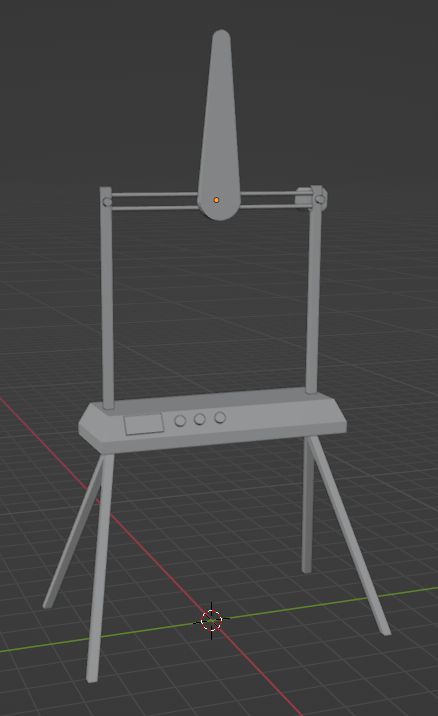
\includegraphics[height=7cm]{Full}
        \end{column}

        \begin{column}{0.48\textwidth}
            \begin{block}{Overview}
                Develop a system that can..
                \begin{enumerate}
                 \item Design
                 \item Train
                 \item Educate
                \end{enumerate}

                On the topic of PID systems.
            \end{block}
        \end{column}
    \end{columns}

    \note{
        \huge Austin \normalsize

        We are building a PID Demonstrator, witch is a tool designed
        to train, educate and sharpen the skills required for engineers
        and operators to train PID loops. Which are a common algorithm
        that drive many modern systems.
    }
\end{frame}

\begin{frame}
    \frametitle{Block Diagram}

    \begin{columns}
        \begin{column}{0.70\textwidth}
            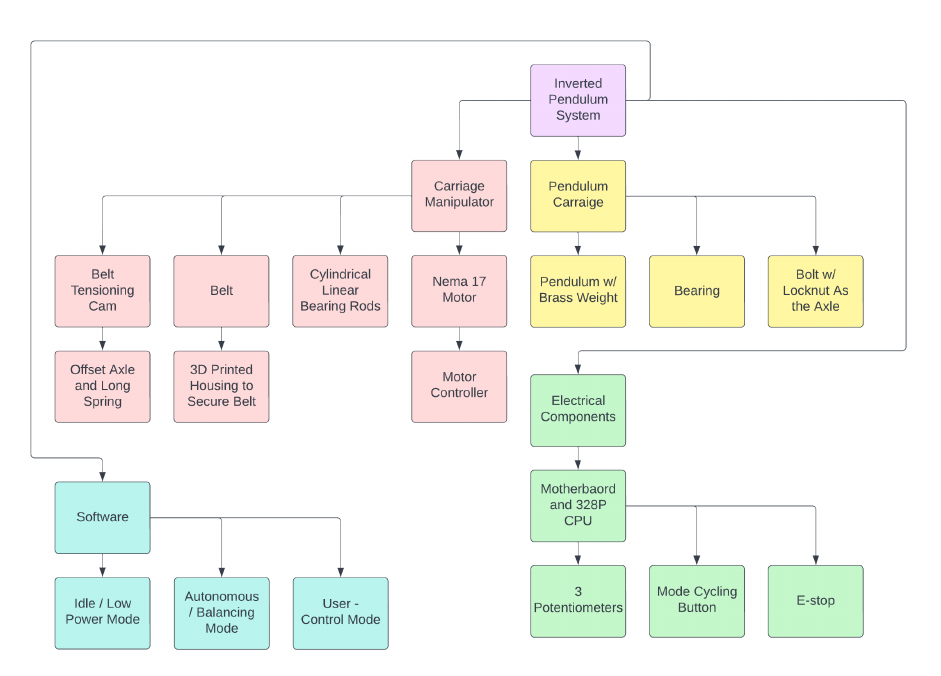
\includegraphics[height=7cm]{BlockDiagram}
        \end{column}

        \begin{column}{0.30\textwidth}
            \begin{block}{Block Diagram}
                The block diagram details the electrical, mechanical and software components and their relationship to each other.
            \end{block}
        \end{column}
    \end{columns}

\note{
\huge Matt \normalsize

\begin{itemize}
 \item Our block diagram shows how our software, hardware and electronics may interact in a final system
\end{itemize}
}

\end{frame}

\begin{frame}
    \frametitle{ConOps Summary}

    \begin{columns}

    \begin{column}{0.34\textwidth}
        Stakeholders
        \begin{itemize}
         \item SNHU
         \item Professors
         \item Industrial Trainers
         \item Parts and manufacturers
        \end{itemize}

        Users
        \begin{itemize}
         \item Pendulum Team
         \item Educators
        \end{itemize}
    \end{column}

    \begin{column}{0.65\textwidth}
        \begin{block}{Operating Modes}
            \begin{enumerate}
            \item Off mode
            \item Idle mode
            \item Spinup mode
            \item Demo mode
            \item User PID mode
            \end{enumerate}
        \end{block}

        \begin{block}{System Description}
            \small{An inverted pendulum is a type of PID Demonstrator, where a simple PID loop
            controls and minimizes the error in a system. In this case, the error is the angle of the pendulum. A perfectly tuned PID loop will hover the pendulum}
            \textbf{perfectly still}.
        \end{block}
    \end{column}
\end{columns}

\note{
\huge Matt \normalsize

\begin{itemize}
 \item So our stakeholders include SNHU, our professors, industrial trainers and of course the people who supply parts and manufacturer our product.
 \item At the moment, we're the ones manufacturing it but in the future it could be different.
 \item Our users are us and educators who might want to use this product to teach the fundamentals of PID
 \item It has a few modes, Off, Idle, Spinup, Demo and user PID mode. The last two are where the pendulum self-balances
 \item Its almost like a game, the system is naturally unstable, the pendulum wants to fall, but a properly tuned PID loop can keep it upright!
\end{itemize}
}

\end{frame}

\begin{frame}
    \frametitle{ConOps (cont.)}

    \begin{columns}
        \begin{column}{0.48\textwidth}
            \begin{block}{Operation and Support Environment}
                \begin{itemize}
                 \item Built from COTS (common off the shelf) parts
                 \item Designed to be serviced
                 \item Constant uptime
                 \item Low power modes
                \end{itemize}
            \end{block}
        \end{column}

        \begin{column}{0.48\textwidth}
            \begin{block}{Impact considerations}
                \begin{itemize}
                 \item Requiring physical space, either for storage or use.
                 \item Being a hazard and risking misuse.
                 \item Generating pollutants and disposal.
                \end{itemize}
            \end{block}
        \end{column}
    \end{columns}

\note{
\huge Matt \normalsize

\begin{itemize}
 \item Being built from COTS parts allows us to easily replace components and design service schedules
 \item We also have plans for a low power mode and folding or removable legs to decrease electrical and physical footprint.
\end{itemize}
}

\end{frame}

\section{Software/Electrical}
\begin{frame}
    \frametitle{The Software/Electrical Subsystem}

    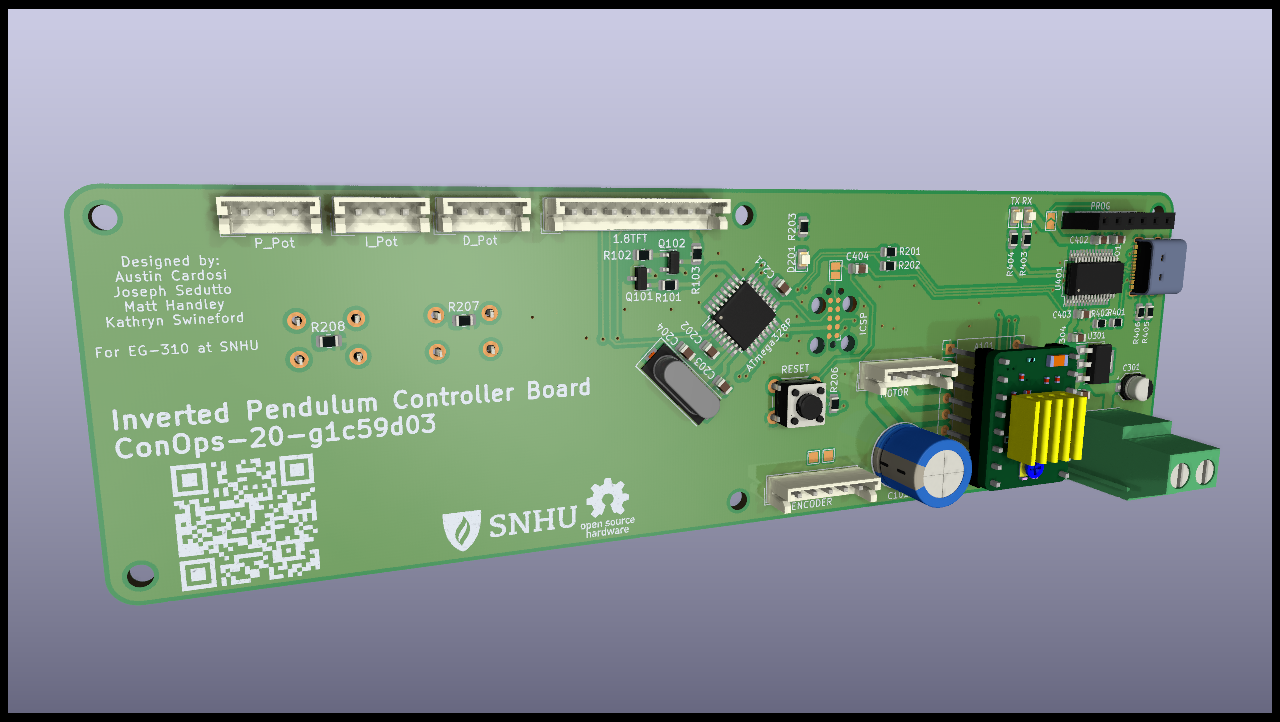
\includegraphics[height=7cm]{CircuitBoard}

    \note{
        \huge Joe \normalsize

        In our system the software and hardware are very closely
        linked.

        We have several features such as the E-Stop that
        rely heavily on an integration between embedded code
        and physical electrical hardware interlocks.
    }
\end{frame}

\begin{frame}
    \frametitle{The Software/Electrical Subsystem (cont.)}

    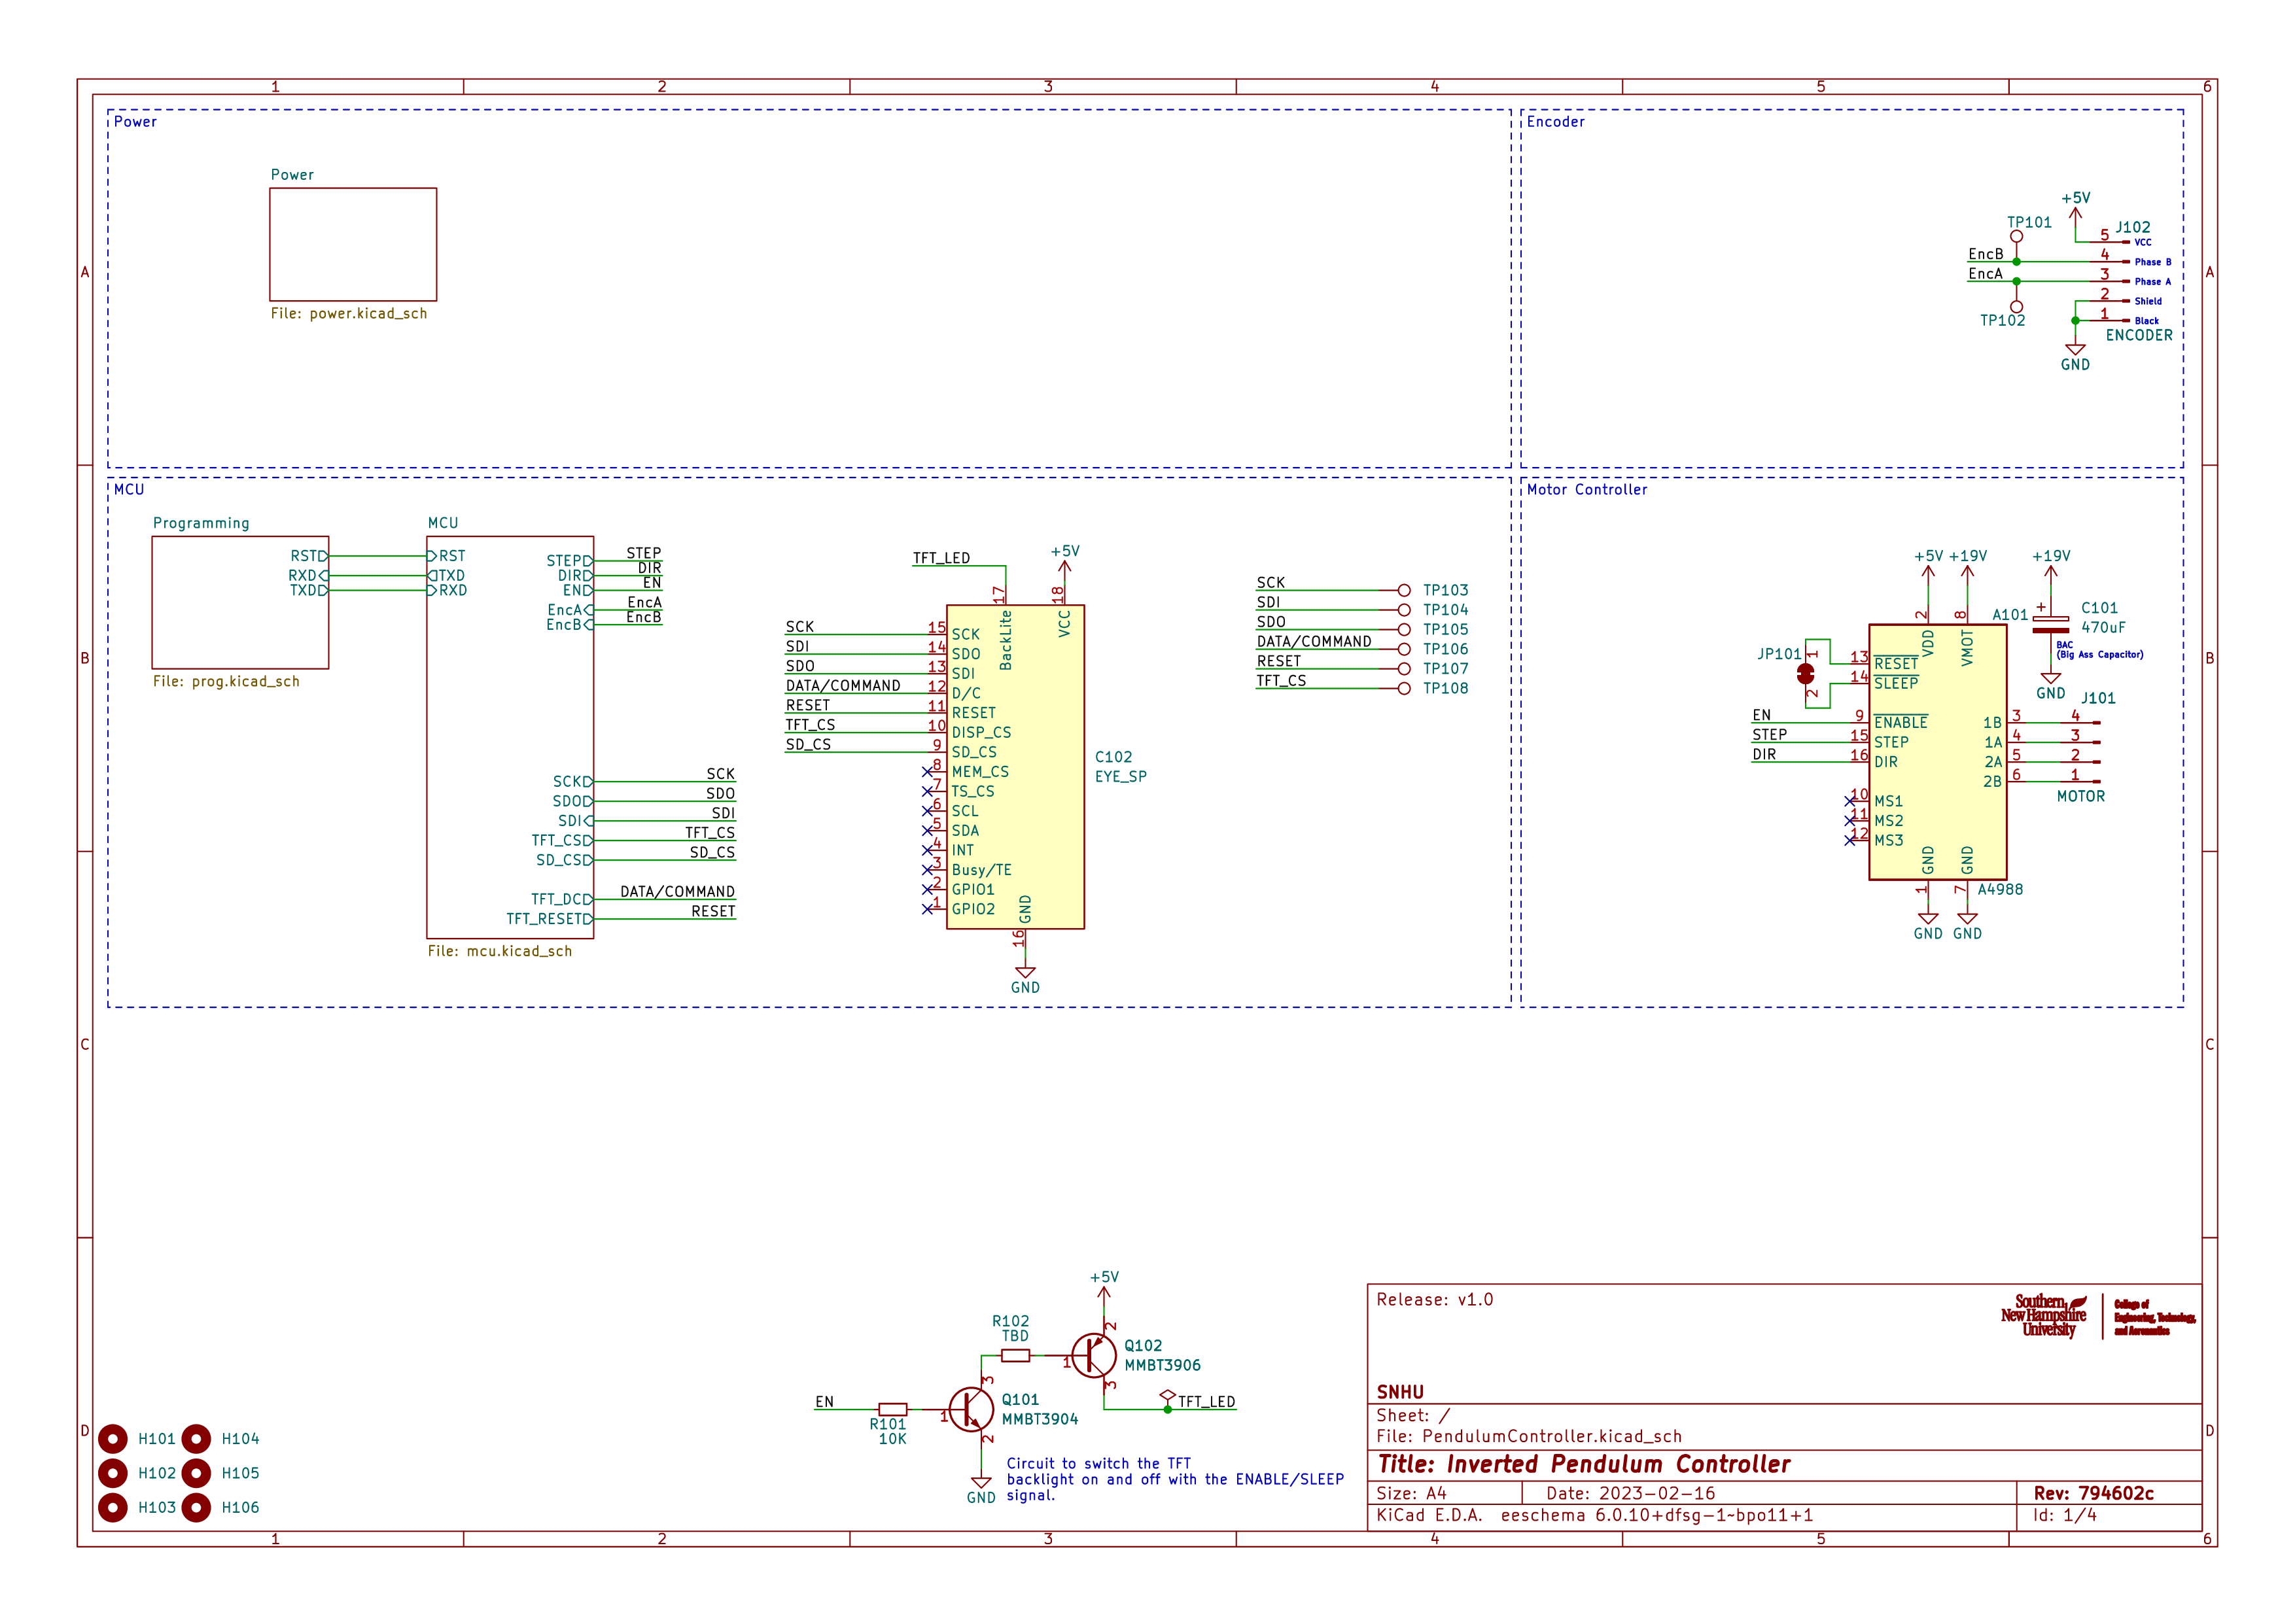
\includegraphics[height=7cm]{Schematic}

    \note{
        \huge Joe \normalsize

        We've designed the general circuitry to take advantage of every
        safety feature the 328p offers such as:
        \begin{enumerate}
         \item A hardware watchdog
         \item Integrated current monitoring
         \item A standby shutdown
         \item And an integrated clock
        \end{enumerate}

    }
\end{frame}

\begin{frame}
    \frametitle{Summary of Trade Studies}

    \begin{columns}
        \begin{column}{0.70\textwidth}
            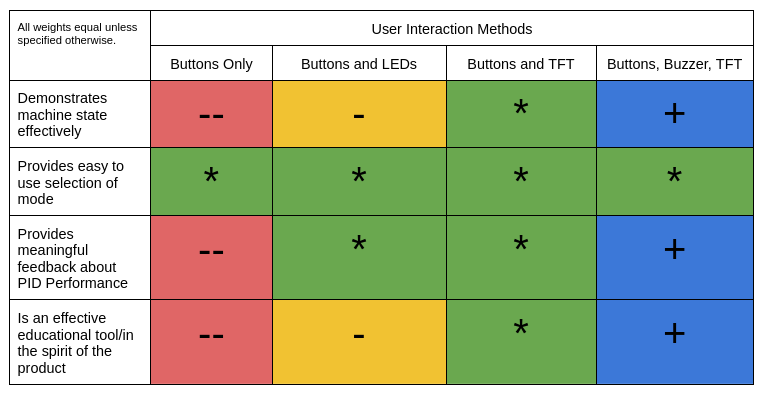
\includegraphics[width=10.5cm]{UserInteractionTradeStudy}
        \end{column}

        \begin{column}{0.28\textwidth}
            \begin{block}{User Interactions}
                The way the user interacts with our system is an important
                part of our design. If the system does not meaningfully
                interact with the operator, then it does not perform
                to our requirements.
            \end{block}
        \end{column}
    \end{columns}

    \note{
        \huge Joe \normalsize

        The way that the user interacts with the system is very important to our project.
        We want a product that will effectively communicate how and why a PID loop
        works.

        Our chart places the TFT plus buzzer, plus buttons as the best for our requirements.
    }
\end{frame}

\begin{frame}
    \frametitle{Summary of Trade Studies (cont.)}

    \begin{columns}
        \begin{column}{0.70\textwidth}
            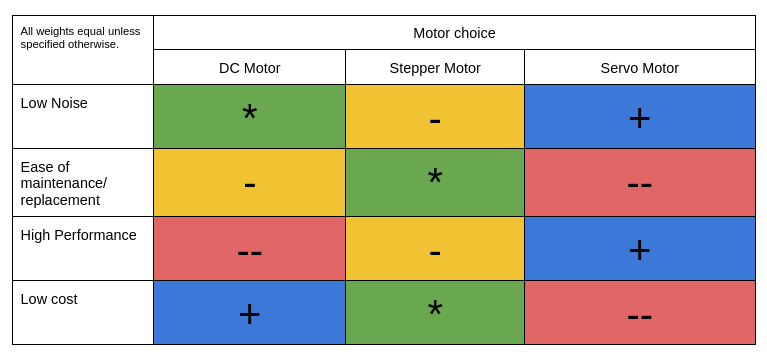
\includegraphics[width=10.5cm]{MotorTradeStudy}
        \end{column}

        \begin{column}{0.28\textwidth}
            \begin{block}{Motors}
                We use our requirements to balance weight, sound
                cost and performance.
            \end{block}
        \end{column}
    \end{columns}

    \note{
        \huge Joe \normalsize

        The motor we choose will affect performance as well as noise and cost. We
        decided to go with a simple stepper motor.
    }
\end{frame}

\begin{frame}
    \frametitle{Software Flowchart}

    \begin{columns}
        \begin{column}{0.72\textwidth}
            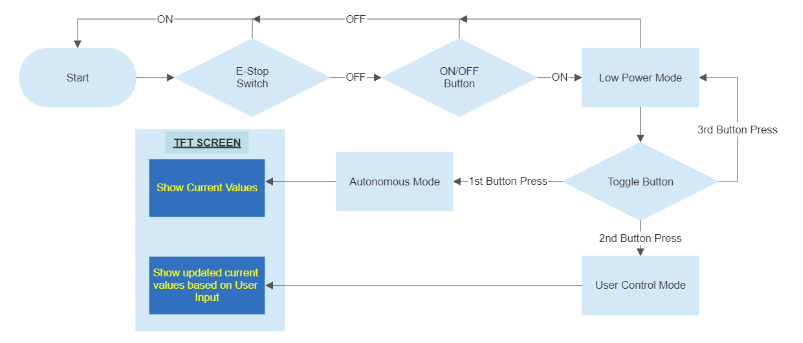
\includegraphics[width=11cm]{Operation}
        \end{column}

        \begin{column}{0.28\textwidth}
            \begin{block}{Software Flowchart}
                The software flowchart is an overview of all the software functions of our
                proposed product.
            \end{block}
        \end{column}
    \end{columns}

\note{
\huge Austin \normalsize

\begin{itemize}
 \item Our software flowchart details how the PID control scheme will be interactable by the users
\end{itemize}
}

\end{frame}

\begin{frame}
    \frametitle{Verification Plan (Electrical/Software)}

    \begin{columns}
        \begin{column}{0.58\textwidth}
            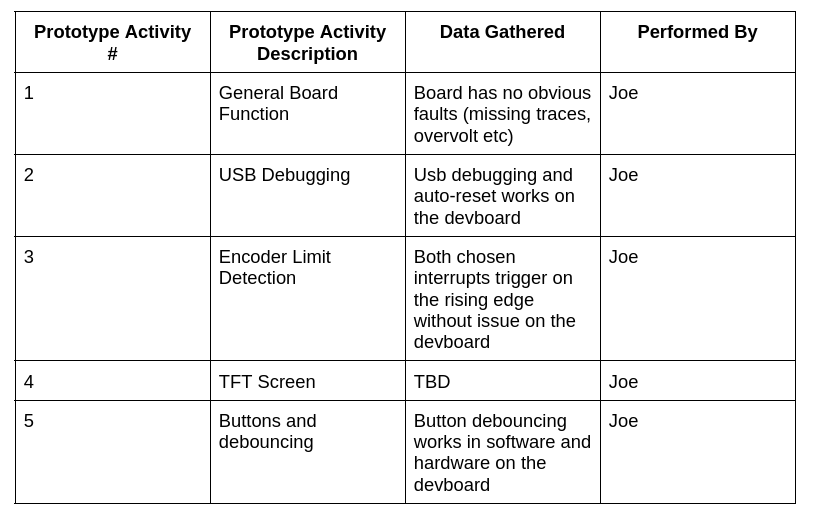
\includegraphics[width=8.5cm]{ElectricalPrototype}
        \end{column}

        \begin{column}{0.40\textwidth}
            \begin{block}{Block Diagram}
                \tiny{
                    Mainboard requires several important features:
                    \begin{enumerate}
                        \item E-Stop
                        \item Button Inputs
                        \item Potentiometers
                        \item Encoder
                        \item Motor output
                        \item Limit Switch
                        \item TFT Screen
                    \end{enumerate}

                    The prototype board implements all these features as well as...
                    \begin{enumerate}
                        \item USB Programming/debugging
                        \item Status lights
                        \item Mode and start select buttons
                        \item Onboard VRM
                    \end{enumerate}
                }
            \end{block}
        \end{column}
    \end{columns}

    \note{
        \huge Austin \normalsize

        The electrical components must adheere to the standards we set
        and must pass our tests

        The most important tests are that the board \textbf{Generally Functions}
        and that we can \textbf{Program and Debug} it without an external
        programmer.
    }
\end{frame}

\section{Mechanical System}
\begin{frame}
    \frametitle{The Mechanical Subsystem}

    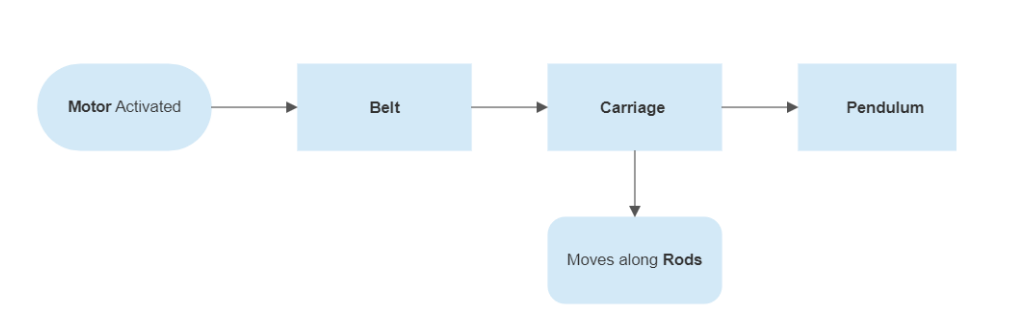
\includegraphics[width=15cm]{MechanicalSubsystem}

    \note{
        \huge Austin \normalsize

        We love you austin!
    }
\end{frame}

\begin{frame}
    \frametitle{System Design}

    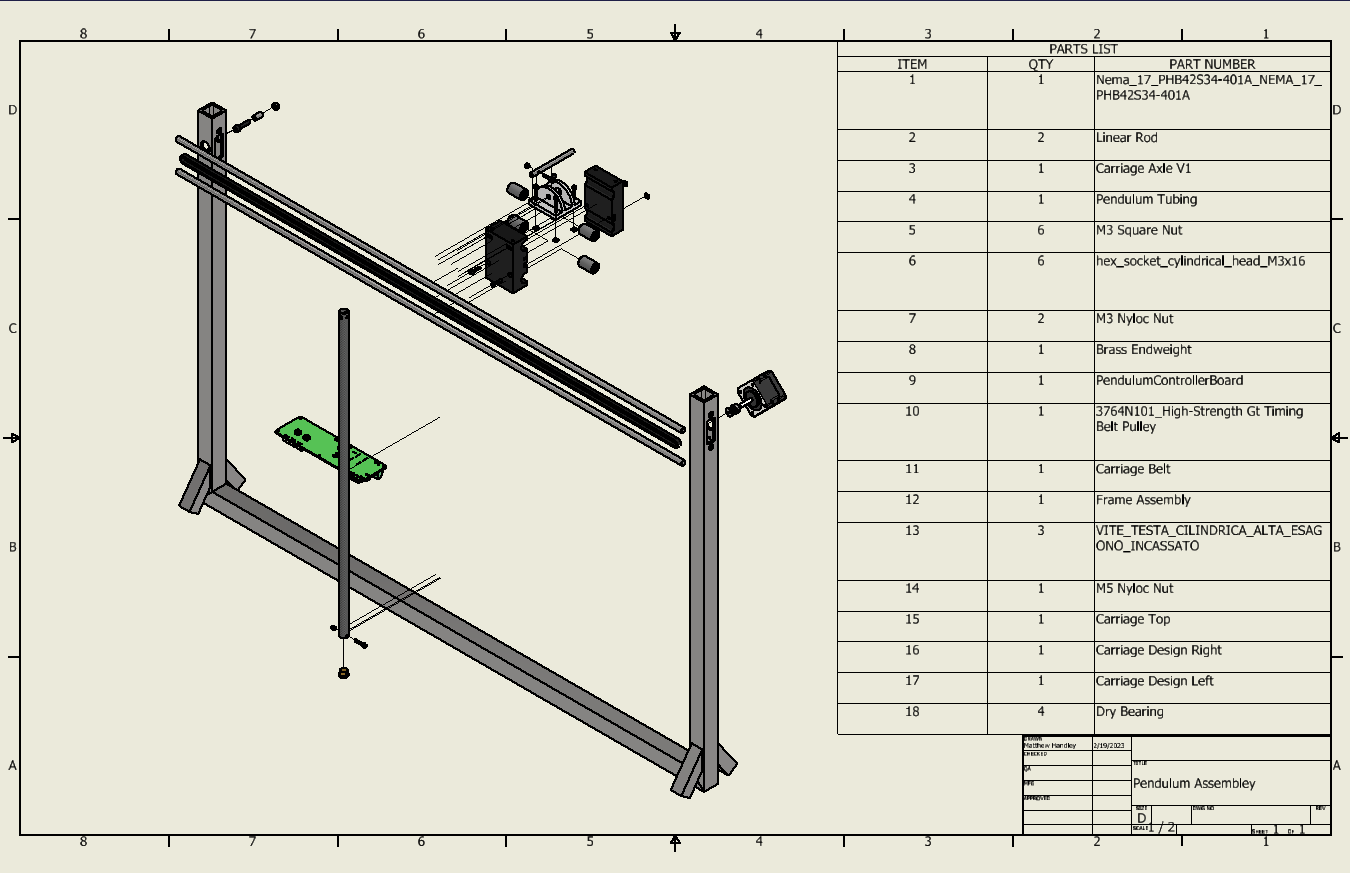
\includegraphics[width=10.5cm]{exploded}

    \note{
        \huge Matt \normalsize

        Note that the tubing contains all cutouts and motor mounts, eliminating
        the need for expensive dedicated brackets and fixtures.
    }
\end{frame}

\begin{frame}
    \frametitle{Summary of Trade Studies}

    \begin{columns}
        \begin{column}{0.28\textwidth}
            \begin{block}{Bearings}
                Choosing bearings that meet our minimum requirements
                helps us to design a system that meets the needs we
                expect to solve.
            \end{block}
        \end{column}

        \begin{column}{0.70\textwidth}
            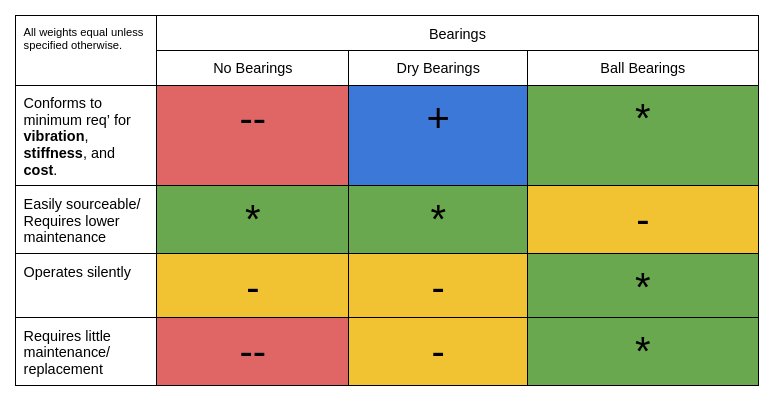
\includegraphics[width=10.5cm]{BearingsTradeStudy}
        \end{column}
    \end{columns}

    \note{
        \huge Matt \normalsize

        To meet the minimum Requirements we've outlined our bearings must be
        \begin{itemize}
         \item Inexpensive
         \item Quiet
         \item and must support the weight of the carriage
        \end{itemize}
    }
\end{frame}

\begin{frame}
    \frametitle{Summary of Trade Studies (cont.)}

    \begin{columns}
        \begin{column}{0.28\textwidth}
            \begin{block}{Material Choice}
                Each material has pros and cons.
            \end{block}
        \end{column}

        \begin{column}{0.70\textwidth}
            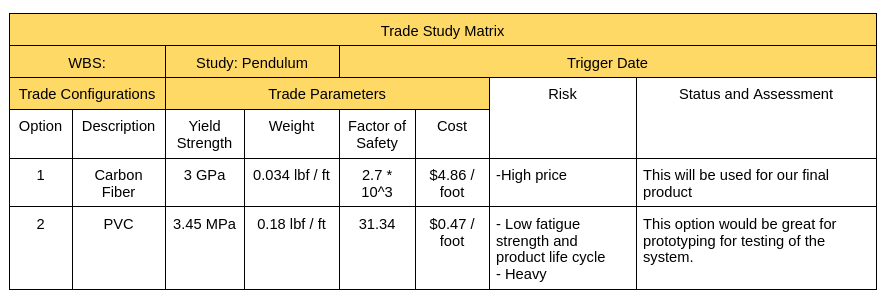
\includegraphics[width=10.5cm]{MaterialTradeStudy}
        \end{column}
    \end{columns}

    \note{
        \huge Matt \normalsize

        The material choice affects cost as well as weight, noise and performance.
    }
\end{frame}

\begin{frame}
    \frametitle{Summary of Trade Studies (cont.)}

    \begin{columns}
        \begin{column}{0.70\textwidth}
            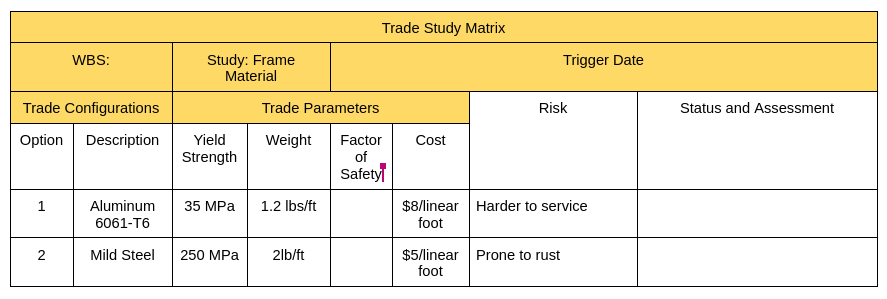
\includegraphics[width=10.5cm]{MetalTradeStudy}
        \end{column}

        \begin{column}{0.28\textwidth}
            \begin{block}{Metal}
                The metal we select affects safety and cost.
            \end{block}
        \end{column}
    \end{columns}

    \note{
        \huge Matt \normalsize

        Idk, wing it man
    }
\end{frame}

\begin{frame}
    \frametitle{Summary of Trade Studies (cont.)}

    \begin{columns}
        \begin{column}{0.28\textwidth}
            \begin{block}{NEMA Motor Choice}
                The specific type of stepper motor impacts strngth and idle power.
            \end{block}
        \end{column}

        \begin{column}{0.70\textwidth}
            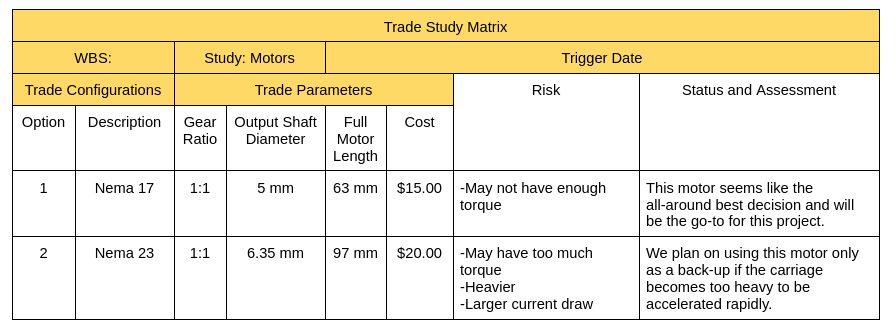
\includegraphics[width=10.5cm]{MotorTradeStudy2}
        \end{column}
    \end{columns}

    \note{
        \huge Matt \normalsize
    }
\end{frame}

\begin{frame}
    \frametitle{Operations}

    \begin{columns}
        \begin{column}{0.30\textwidth}
            \begin{block}{Operations}
                The Operations diagram details the physical and general controls.
            \end{block}
        \end{column}

        \begin{column}{0.70\textwidth}
            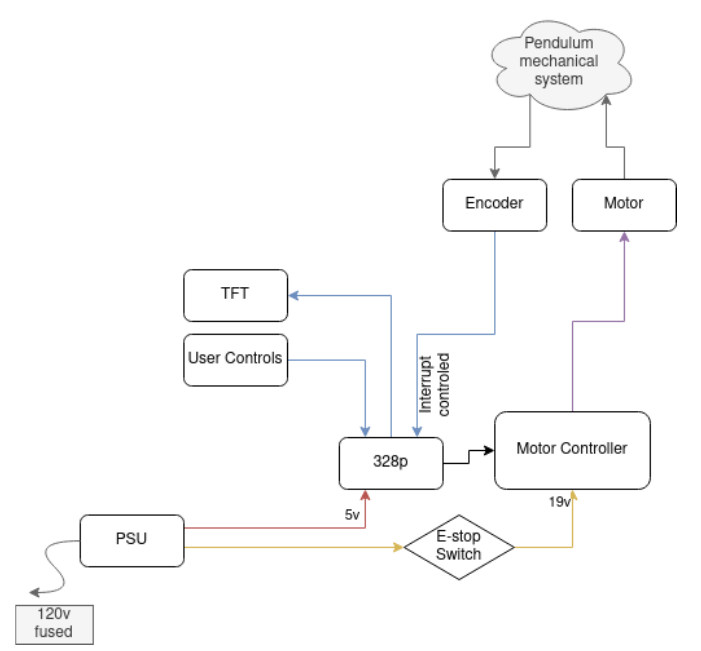
\includegraphics[height=7cm]{Operations}
        \end{column}
    \end{columns}

\note{
\huge Joe \normalsize

\begin{itemize}
 \item The operations chart details our physical and general controls like the tft screen
 \item the buttons
 \item the motor controller and encoders
\end{itemize}
}

\end{frame}

\begin{frame}
    \frametitle{Verification Plan (Mechanical)}

    \begin{columns}
        \begin{column}{0.40\textwidth}
            \begin{block}{Block Diagram}
                \tiny{
                    Each bearing is tested and evaluated with the above chart, with specific attention to:
                    \begin{enumerate}
                        \item Cost of bearing (4 needed for every pendulum)
                        \item Noise (Minimize sliding grinding noises)
                        \item Performance (How well does it slide and protect the carriage shafts)
                        \item Longevity (How long does it last without service or lube?)
                    \end{enumerate}
                }
            \end{block}
        \end{column}

        \begin{column}{0.58\textwidth}
            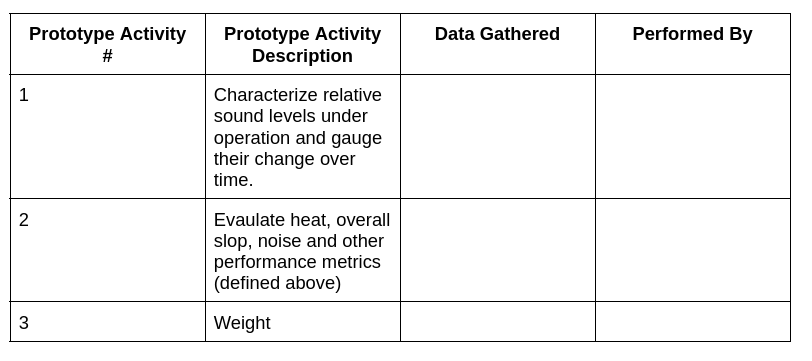
\includegraphics[width=8.5cm]{MechanicalPrototype}
        \end{column}
    \end{columns}

    \note{
        \huge Matt \normalsize
    }
\end{frame}

\section{Requirements}
\begin{frame}
    \frametitle{Functional Requirements}

    \begin{columns}
        \begin{column}{0.70\textwidth}
            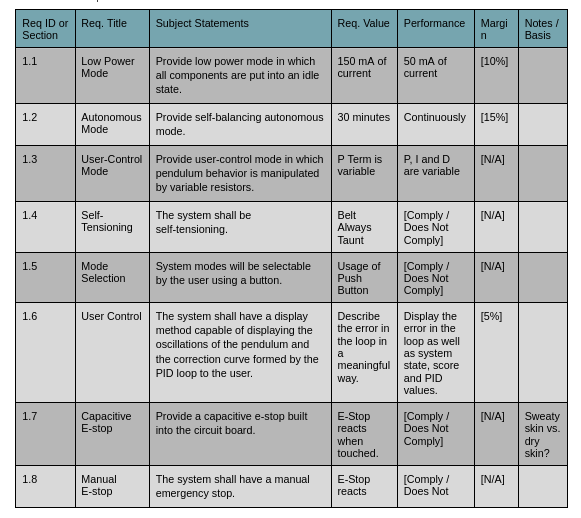
\includegraphics[height=7cm]{Functional1}
        \end{column}

        \begin{column}{0.28\textwidth}
            \begin{block}{Functional Requirements}
                Many of our functional requirements include features such as
                a different modes and mode slections. As well as limits on
                weight, power draw and assembly time.
            \end{block}
        \end{column}
    \end{columns}

    \note{
        \huge Matt \normalsize
    }
\end{frame}

\begin{frame}
    \frametitle{Functional Requirements (cont.)}

    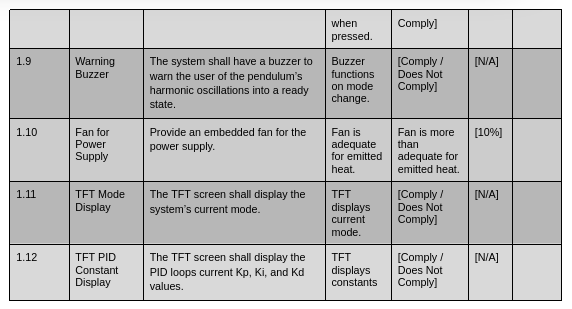
\includegraphics[height=7cm]{Functional2}

    \note{
        \huge Joe \normalsize
    }
\end{frame}

\begin{frame}
    \frametitle{Performance Requirements}

    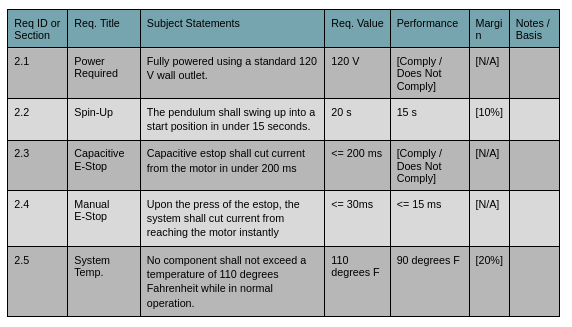
\includegraphics[height=7cm]{Performance}

    \note{
        \huge Austin \normalsize

        We'll need to meed specific functional requirements like displaying
        the mode and keeping the power supply cool.
    }
\end{frame}


\begin{frame}
    \frametitle{Interface and Design Requirements}

    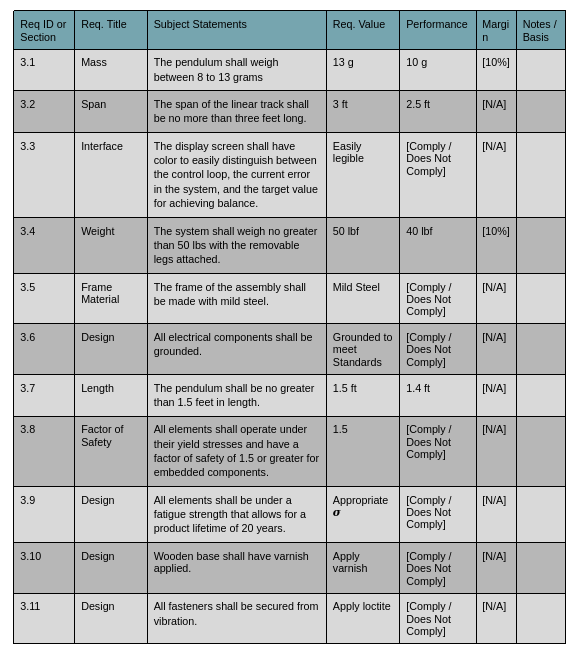
\includegraphics[height=7cm]{OtherReqs}

    \note{
        \huge Joe \normalsize

        We'll need to inteface to existing infrastructure such as
        120v AC and have standardized e-stop technology
    }
\end{frame}


\section{Design}
\begin{frame}
    \frametitle{Bill Of Materials}

    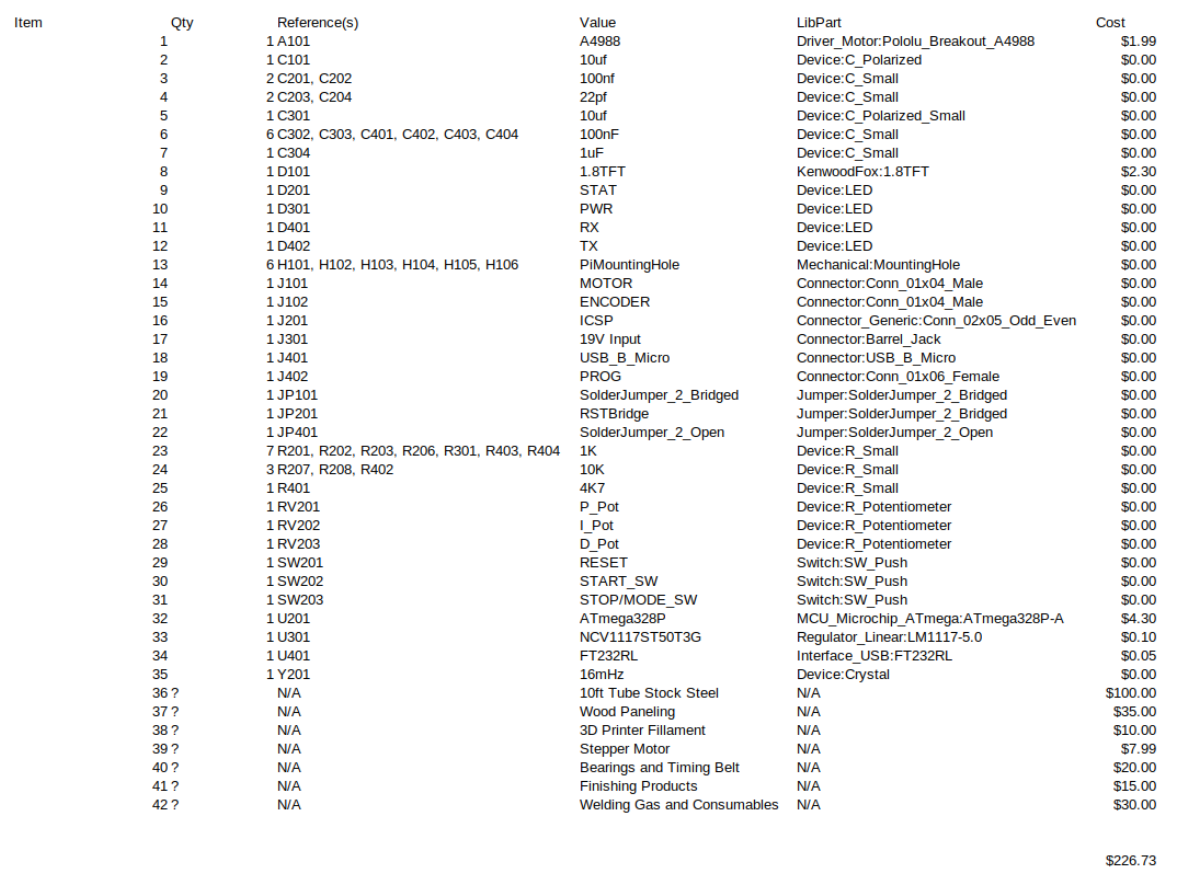
\includegraphics[height=7cm]{BOMTable}

    \note{
        \huge Matt \normalsize

        Our bill of materials is very long but everything is here even down
        to the smallest individual components.
    }
\end{frame}

\begin{frame}
    \frametitle{Ordering Status}

    \begin{block}{Bearings}
        Dry bearings have arrived, ball bearings still in mail.
    \end{block}

    \begin{block}{PCB}
        PCB Confirmed Ordered.
    \end{block}

    \begin{block}{Steel}
        We're in the process of sourcing steel.
    \end{block}

    \begin{block}{3D/plastic/COTS}
        Material stock for welding, 3D printing and machining are ready to go.
    \end{block}

    \note{
        \huge Matt \normalsize
    }
\end{frame}


\begin{frame}
    \frametitle{Impact Considerations}

    \begin{enumerate}
        \item Being a hazard and risking misuse.
        \item Requiring physical space, either for storage or use.
        \item The system will generate waste at the end of its life cycle. The goal is to minimize this waste through the use of recyclable materials
    \end{enumerate}

    \note{
        \huge Austin \normalsize
    }
\end{frame}

\section{Calibration and Maintenance}
\begin{frame}
    \frametitle{Calibration and Maintenance}

        \begin{itemize}
            \item Self test and Auto Calibration
            \item Use of hardware limits
            \item Torque specs for all fasteners
            \item Published maintenance schedule in docs.
        \end{itemize}

    \note{
        \huge Austin \normalsize

        \begin{enumerate}
        \item The system shall perform a self-test on start-up. Due to the pendulum hanging towards the center of the earth due to gravity, the encoder on the pendulum will be zeroed using the position.
        \item The motor shall move towards a limit switch at a set slow speed until it triggers one of the two limit switches on either side of the linear rails, upon triggering one, the carriage will then move a set amount of motor steps to the middle of the span of the linear rails.
        \item All fasteners shall have their tightness ensured before operation, and any renewal of lubrical for the pendulum shall be performed.
        \item A maintenance and component replacement manual shall be created in order to easily explain how to replace the COTS (common of the shelf) parts such as the precision belt or the motor internals.
    \end{enumerate}
    }
\end{frame}

\begin{frame}
    \frametitle{Safety}

    \begin{itemize}
     \item Electrical
        \begin{itemize}
         \item E-Touch - Capacitive sensor that detects when a user has provided a static charge or short circuit and will automatically turn off the power
        \end{itemize}

    \item Software
        \begin{itemize}
         \item Limits -  Designed to restrict the upper bounds of the provided commands and to make sure the acceleration and velocities don't exceed a maximum.
        \end{itemize}

    \item Mechanical
        \begin{itemize}
            \item Emergency Stop - When pressed ON all electronics will have receive NO electric flow
            \item Protective Shield - Shield designed to protect operators from pinch points created by the movement of the carriage along the rods.
            \item Buzzer - Designed to warn the operator when the system is in autonomous “swing up” mode using harmonic oscillations
            \item Power light - The system will have an LED to indicate when it is receiving power
            \item TFT Screen - The TFT screen will display what mode the system is currently running so the operator is aware.
        \end{itemize}
    \end{itemize}

    \note{
        \huge Safety \normalsize

        Most important features are sheilding

        capactive estop

        grounding

        access to cleaning to remove dust and prevent overheating
    }
\end{frame}

\begin{frame}
    \frametitle{Phase D}

    \begin{enumerate}
        \item All drawings and assemblies are on the latest revision and meet all specifications
        \item All required parts will be ordered through Carlstrom / Joe Donovan this week (2/22/2023)
        \item Manufacturing of the frame will begin as soon as the steel is delivered, and prototyping of parts will begin once all remaining parts are delivered.
        \item Drawings and assemblies will be finalized this weekend (2/25/2023) for machining to begin.
    \end{enumerate}


    \note{
        \huge Joe \normalsize
    }
\end{frame}

\begin{frame}
    \frametitle{End}

    \begin{block}{}
        \begin{center}
            \Huge Questions and Comments?
        \end{center}
    \end{block}

    \begin{center}
        Find the source code for this document, and the rest of our designs, firmware, hardware
        and notes on GitHub!

        
\includegraphics[height=2cm]{github_qr}
    \end{center}

\note{
\begin{itemize}
 \item So please if you have any questions we would love to hear them.
 \item All of our software, CAD, hardware and design docs are licensed under
 \item \huge The MIT Open Source License \normalsize and available via git.
 \item If you have a specific slide in mind we can go back to it!
\end{itemize}
}
\end{frame}

\section{Backup Slides}
\begin{frame}
    \frametitle{Code}

    \begin{columns}
        \begin{column}{0.58\textwidth}
            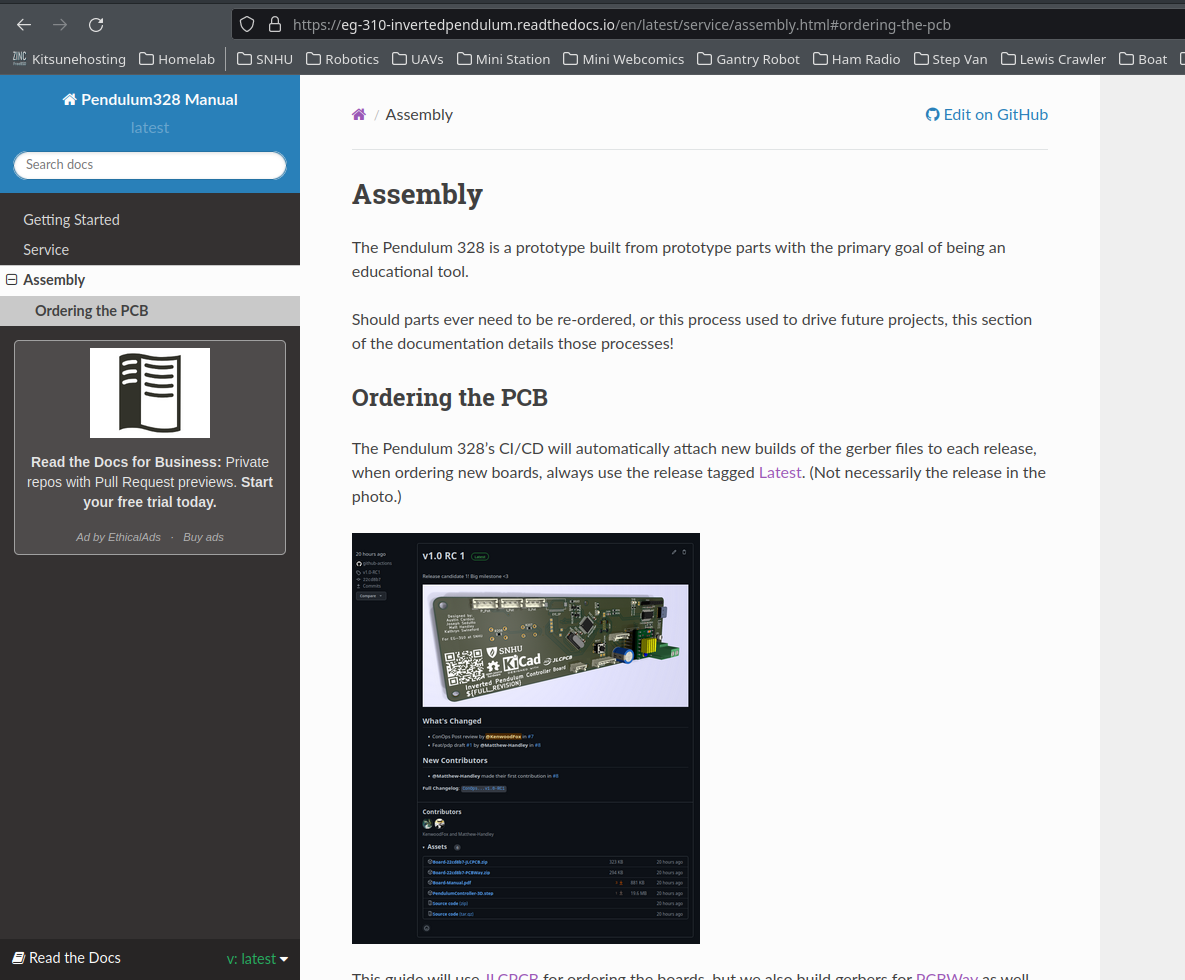
\includegraphics[height=7cm]{ManualOnline}
        \end{column}

        \begin{column}{0.38\textwidth}
            \begin{block}{Our Documentation}
                Find our docs online, built from the very code and CAD that
                makes our project, conforming closely to industry standards
                for industrial automation.
            \end{block}
        \end{column}
    \end{columns}
\end{frame}

\begin{frame}
    \frametitle{Online Colaboration}

    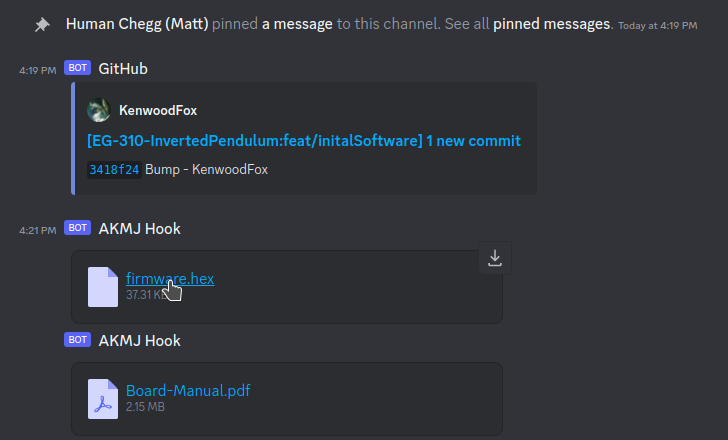
\includegraphics[height=4cm]{DevelopmentDiscouse}

    We use discord and github to faccilatate automatic CAD, Code, and automatic
    CI\/CD as well as..

    \begin{enumerate}
     \item Unit testing
     \item Doc generation
     \item Automated test\/deploy
     \item And project management
    \end{enumerate}
\end{frame}

\begin{frame}
    \frametitle{Carriage}

    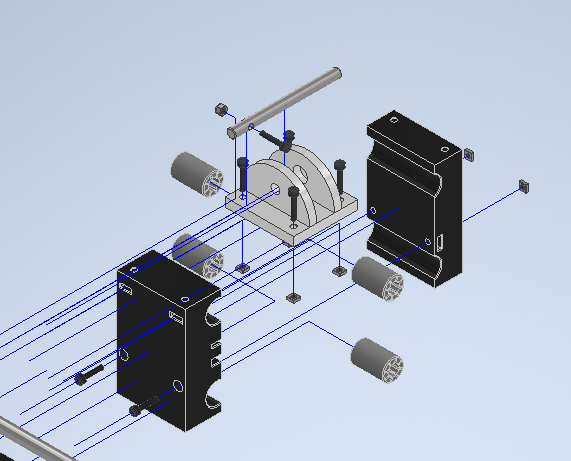
\includegraphics[height=7cm]{closeup1}
\end{frame}

\begin{frame}
    \frametitle{Carriage (cont.)}

    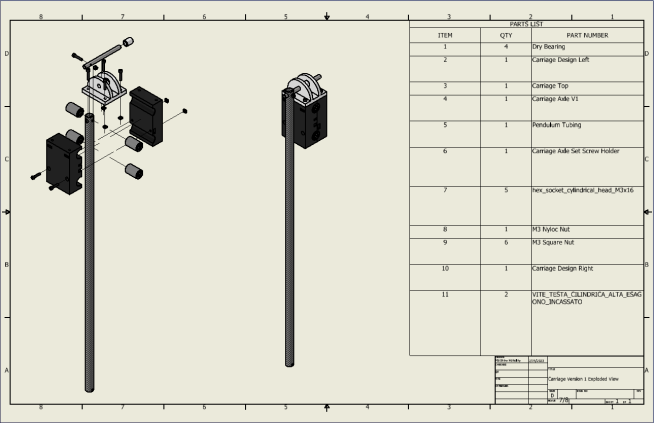
\includegraphics[height=7cm]{closeup2}
\end{frame}

\begin{frame}
    \frametitle{End Section}

    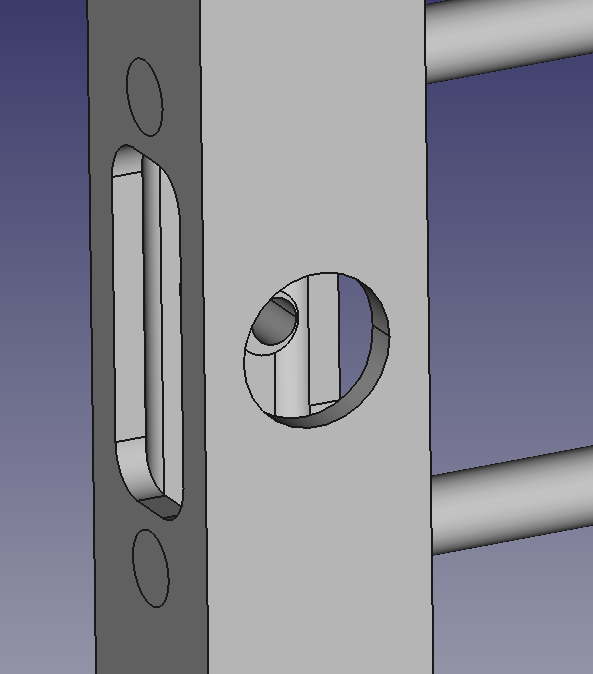
\includegraphics[height=7cm]{closeup3}
\end{frame}

\begin{frame}
    \frametitle{Bezel}

    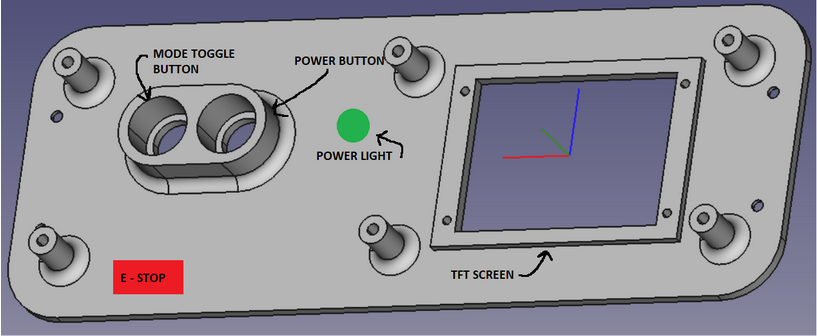
\includegraphics[height=6cm]{closeup4}
\end{frame}

\begin{frame}
    \frametitle{Carriage Render}

    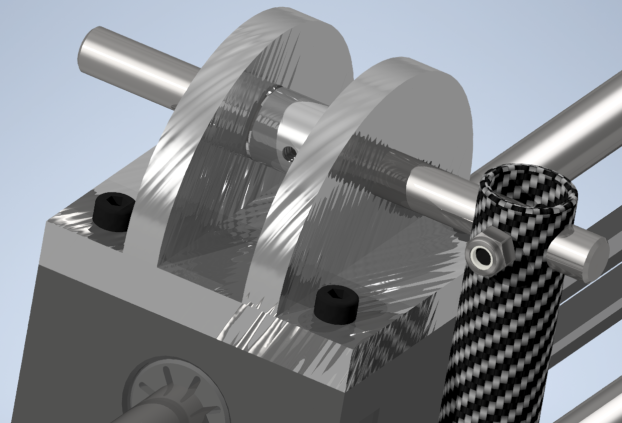
\includegraphics[height=6cm]{closeup5}
\end{frame}

\begin{frame}
    \frametitle{Calculations}

    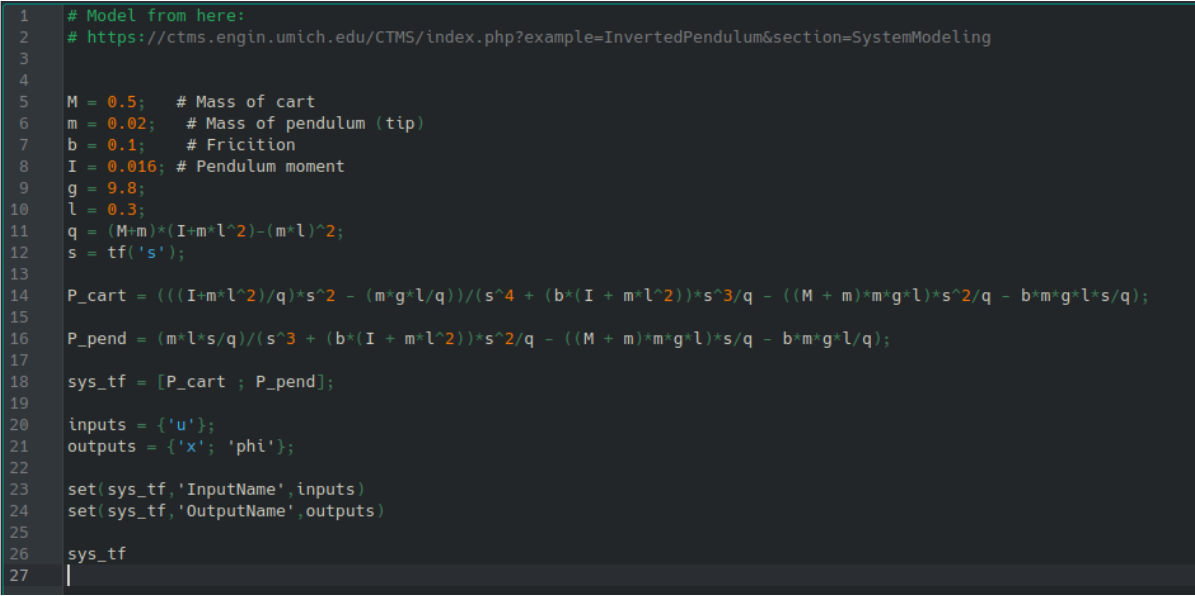
\includegraphics[height=6.5cm]{Calculations}

    Octave math model.
\end{frame}

\begin{frame}
    \frametitle{Calculations (cont.)}

    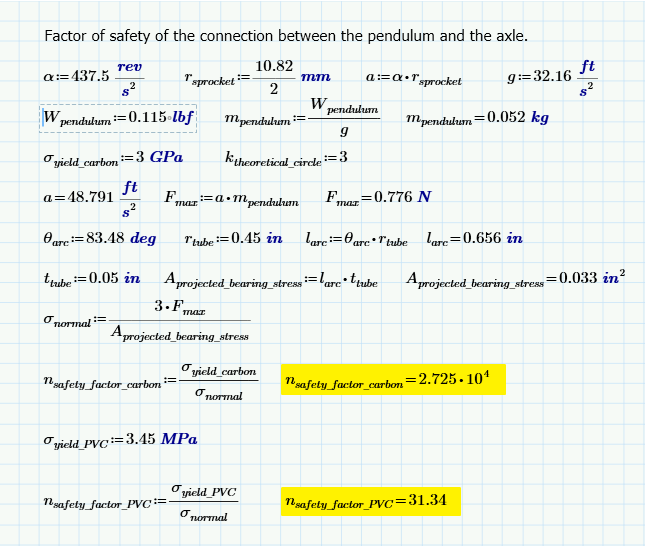
\includegraphics[height=6.5cm]{CalculationsMatt}

    Hand math model.
\end{frame}

\begin{frame}
    \frametitle{Code}

    \begin{columns}
        \begin{column}{0.48\textwidth}
            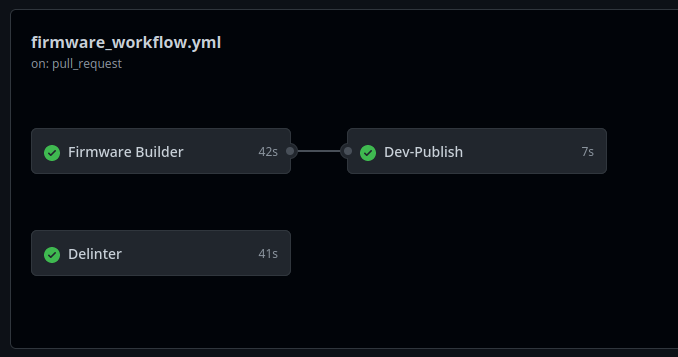
\includegraphics[width=6.5cm]{CodePasses}
        \end{column}

        \begin{column}{0.48\textwidth}
            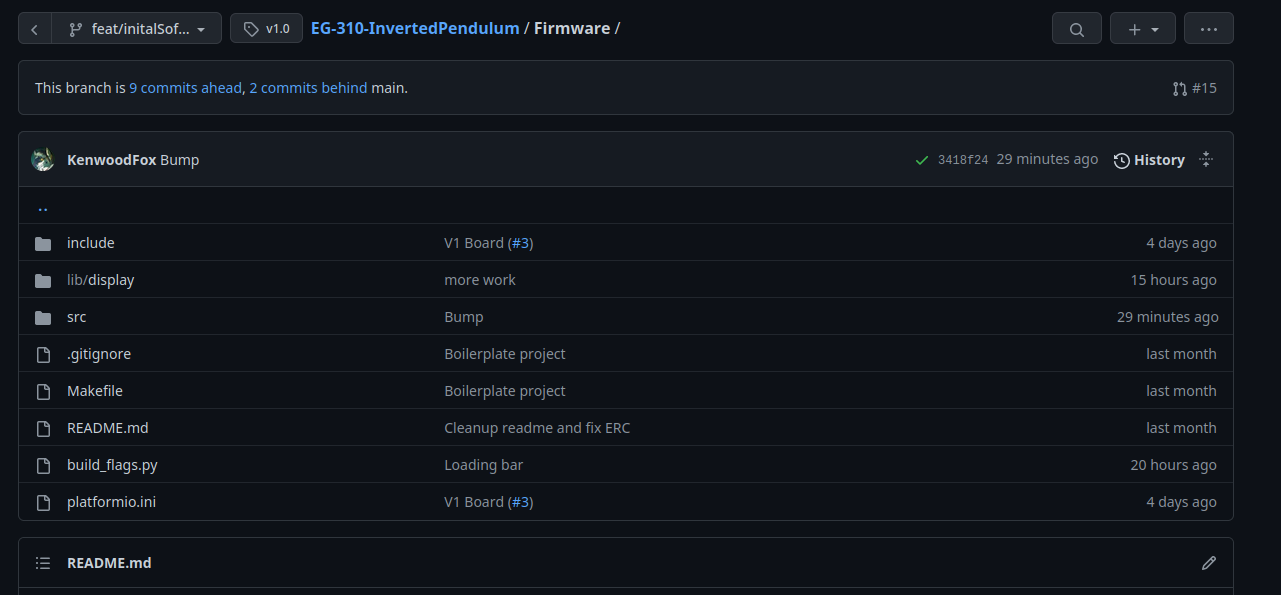
\includegraphics[width=6.5cm]{CodeOnline}
        \end{column}
    \end{columns}
\end{frame}

\begin{frame}
    \frametitle{References}

    
\includegraphics[width=12cm]{CDRReferences}
\end{frame}

\end{document}
